\documentclass[../main.tex]{subfiles}

\begin{document}

\section{Problem 1}

Plot the photon number distribution $p(n)=\abs{\braket{n}{\psi}}^2$ of a coherent state $\ket{\alpha}$, a Fock state, and a single-mode thermal state for $\expval{n}=1,10$ and $100$ (9 plots in total).
For each additionally provide $\Delta n$ and the most probable outcome of the photon number measurement.

\subsection{Coherent state}

We start by computing the inner product of the coherent state with the $\ket{n}$ state,
\begin{align*}
    \braket{n}{\alpha} &= \bra{n}\qty(\exp\qty[-\frac{\abs{\alpha}^2}{2}]\sum_{m=0}^\infty\frac{\alpha^m}{\sqrt{m!}}\ket{m}) \\
    &= \exp\qty[-\frac{\abs{\alpha}^2}{2}]\sum_{m=0}^\infty\frac{\alpha^m}{\sqrt{m!}}\braket{n}{m} \\
    &= \exp\qty[-\frac{\abs{\alpha}^2}{2}]\sum_{m=0}^\infty\frac{\alpha^m}{\sqrt{m!}}\delta_{n,m} \\
    &= \frac{\alpha^n}{\sqrt{n!}}\exp\qty[-\frac{\abs{\alpha}^2}{2}].
\end{align*}
Now we can compute the squared module by multiplying the inner product with its complex conjugate,
\begin{align*}
    \abs{\braket{n}{\psi}}^2 &= \braket{n}{\alpha}\braket{n}{\alpha}^* \\
    &= \qty[\frac{\alpha^n}{\sqrt{n!}}\exp\qty[-\frac{\abs{\alpha}^2}{2}]]\qty[\frac{\alpha^n}{\sqrt{n!}}\exp\qty[-\frac{\abs{\alpha}^2}{2}]]^*\\
    &= \frac{\alpha^n\alpha^{n*}}{\sqrt{n!}\sqrt{n!}^*}
    \exp\qty[-\frac{\abs{\alpha}^2}{2}-\frac{\abs{\alpha}^2}{2}] \\
     &= \frac{\abs{\alpha}^{2n}}{n!}\exp\qty[-\abs{\alpha}^2].
\end{align*}
If we set $\lambda=\abs{\alpha}^2$, we can rewrite the expression as \[\abs{\braket{n}{\psi}}^2=\frac{\lambda^{n}}{n!}e^{-\lambda}.\]
Hence, we can say that the photon number distribution of a coherent state is represented by a Poisson distribution with $\lambda=\abs{\alpha}^2$.
Since the Poisson distribution is a well-known distribution, we know that the expected value and the variance are equal to $\lambda$.
Therefore, $\Delta n=\abs{\alpha}$.
Those properties can also be obtained using Dirac notation and with the following properties $\hata\ket{\alpha}=\alpha\ket{\alpha},~\bra{\alpha}\hatad=\bra{\alpha}\alpha^*,~\hata\hatad=1+\hatad\hata$,
\begin{align*}
    \Delta\hat{n}^2 &= \expval{\hat{n}^2} - \expval{\hat{n}}^2 \\ 
                    &= \expval{\qty(\hatad\hata)\qty(\hatad\hata)}{\alpha} - \qty(\expval{\hatad\hata}{\alpha})^2 \\
                    &= \expval{\hatad\qty(\hata\hatad)\hata}{\alpha} - \qty(\alpha^*\cancelto{1}{\braket{\alpha}}\alpha)^2 \\
                    &= \alpha^*\expval{1+\hatad\hata}{\alpha}\alpha - \qty(\abs{\alpha}^2)^2 \\
                    &= \abs{\alpha}^2\qty(\cancelto{1}{\braket{\alpha}}+\expval{\hatad\hata}{\alpha}) - \abs{\alpha}^4 \\
                    &= \abs{\alpha}^2\qty(1+\alpha^*\cancelto{1}{\braket{\alpha}}\alpha) - \abs{\alpha}^4 \\
                    &= \abs{\alpha}^2\qty(1+\abs{\alpha}^2) - \abs{\alpha}^4 \\
                    &= \abs{\alpha}^2.
\end{align*}
This confirms that the expected value is $\abs{\alpha}^2$ and that the standard deviation is $\abs{\alpha}.$

\begin{figure}[ht!]
    \centering
    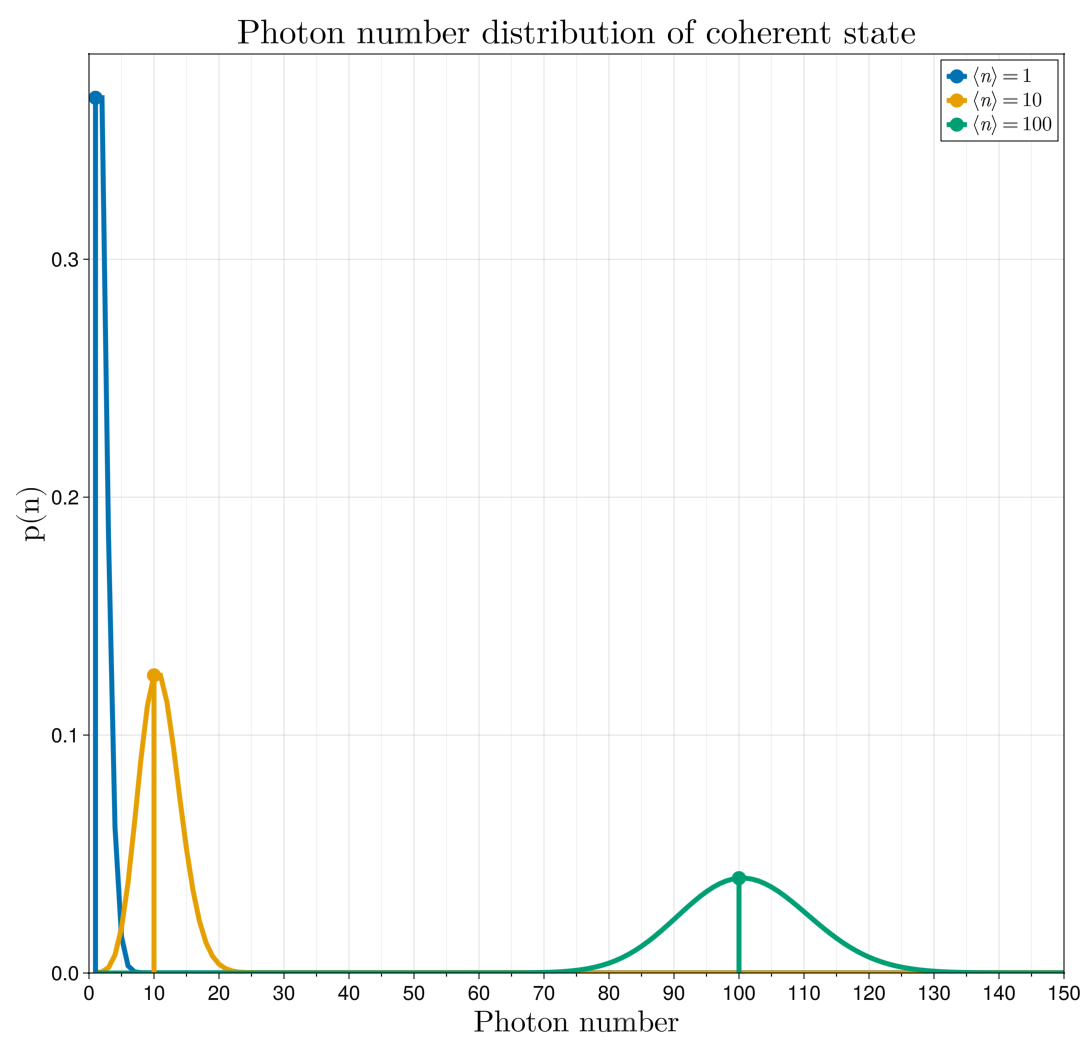
\includegraphics[width=0.8\textwidth]{imgs/fig_coherent.png}
    %\caption{Caption}
    %\label{fig:enter-label}
\end{figure}

\subsection{Fock state}

We repeat the same procedure for the coherent state $\ket{\alpha}$ with the Fock state $\ket{m}$,
\begin{align*}
    \abs{\braket{n}{m}}^2 &= \braket{n}{m}\braket{n}{m}^* \\
    &= \delta_{n,m}\delta_{n,m}^* \\
    &= \delta_{n,m}.
\end{align*}
From this result we can say that the photon number distribution of a Fock state is a Dirac Delta function.
Using the definition of the Dirac Delta function, the expected value of $p(n)$ is $n$.
Therefore, the standard deviation follows as $\Delta n = 0$.
As before, the standard deviation of the distribution and the expected values can be computed using Dirac notation and the following results $\hata\ket{n}=\sqrt{n}\ket{n-1},~\hatad\ket{n}=\sqrt{n+1}\ket{n+1},~\bra{n}\hatad=\bra{n-1}\sqrt{n}^*,~\bra{n}\hata=\bra{n+1}\sqrt{n+1}^*$,
\begin{align*}
    \Delta\hat{n}^2 &= \expval{\hat{n}^2} - \expval{\hat{n}}^2 \\ 
                    &= \expval{\qty(\hatad\hata)\qty(\hatad\hata)}{n} - \qty(\expval{\hatad\hata}{n})^2 \\
                    &= \sqrt{n}^*\expval{\hata\hatad}{n-1}\sqrt{n} - \qty(\sqrt{n}^*\cancelto{1}{\braket{n-1}}\sqrt{n})^2 \\
                    &= n\qty(\sqrt{n-1+1}^*\cancelto{1}{\braket{n-1+1}}\sqrt{n-1+1}) - \qty(n)^2 \\
                    &= n^2 - n^2 \\
                    &= 0.
\end{align*}
This confirms that the expected value is $n$ and that the standard deviation is $0.$

\begin{figure}[ht!]
    \centering
    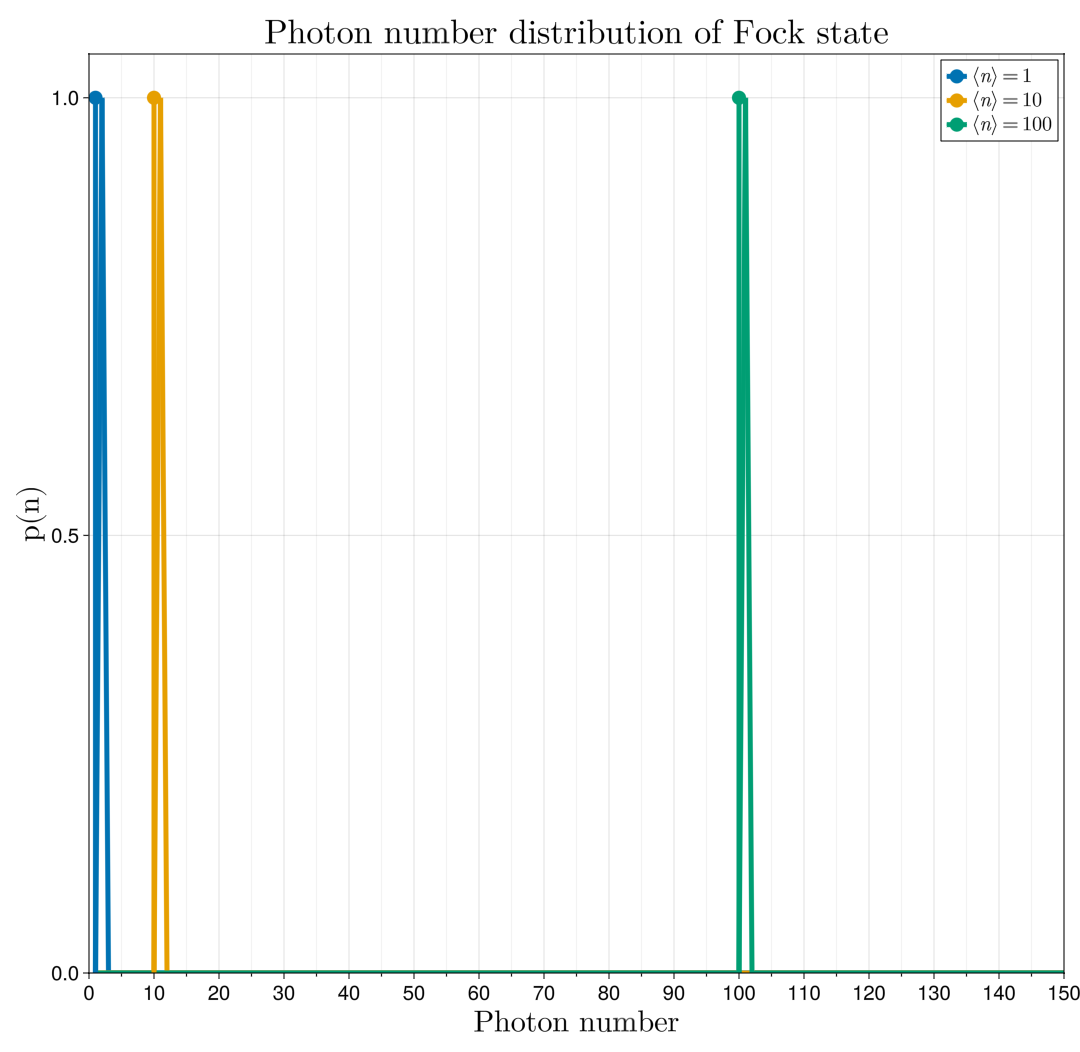
\includegraphics[width=0.8\textwidth]{imgs/fig_fock.png}
    %\caption{Caption}
    %\label{fig:enter-label}
\end{figure}


\subsection{Single-mode thermal state}

Finally, to compute the photon number distribution and the standard deviation of a single-mode thermal state, we are going to use the density matrix framework.
In this framework, the thermal state is represented as follows
\begin{gather*}
    \hat{\rho}_{\mathrm{Th}} = \frac{\exp\qty[-\hat{H}/k_BT]}{\Tr\qty(\exp\qty[-\hat{H}/k_BT])}.
\end{gather*}
Taking into account that we are analyzing a single-mode state, the Hamiltonian can be expressed as $\hat{H}=\hbar\omega\qty(\hat{n}+1/2)$.
First we compute the trace,
\begin{align*}
    \Tr\qty(\exp\qty[-\frac{\hat{H}}{k_BT}]) &= \sum_{n=0}^\infty\expval{\exp\qty[-\frac{\hat{H}}{k_BT}]}{n} \\
    &= \sum_{n=0}^\infty\exp\qty[-\frac{E_n}{k_BT}]
\end{align*}
where $E_n=\hbar\omega\qty(n+1/2)$.
Since the density matrix needs to be normalized, the trace is the normalization coefficient, which is also known as the partition function $Z$.
This partition function for single-mode thermal light is
\begin{gather*}
    Z = \exp\qty[-\frac{\hbar\omega}{2k_BT}]\sum_{n=0}^\infty\exp\qty[-\frac{\hbar\omega n}{k_BT}].    
\end{gather*}
Considering $\qty(\hbar\omega)/\qty(2k_BT)<1$, we can approximate the sum of the partition function as a geometric series,
\begin{gather*}
    Z = \frac{\exp\qty[-\hbar\omega/2k_BT]}{1-\exp\qty[-\hbar\omega /k_BT]}.    
\end{gather*}

Rewriting the expression of the density matrix for the thermal state using the partition function, we get,
\begin{align*}
    \hat{\rho}_{\mathrm{Th}}    &= \frac{1}{Z}\exp\qty[-\hat{H}/k_BT] = \frac{1}{Z}\exp\qty[-\hbar\omega\qty(\hat{n}+1/2)/k_BT]. %\\
                                %&= \frac{1-\exp\qty[-\hbar\omega /k_BT]}{\exp\qty[-\hbar\omega/2k_BT]} \exp\qty[-\hbar\omega\qty(\hat{n}+1/2)/k_BT] \\
                                %&= \qty(1-\exp\qty[-\frac{\hbar\omega}{k_BT}]) \exp\qty[-\frac{\hbar\omega\hat{n}}{k_BT}] \\
\end{align*}

Now that we know the partition function we can compute the photon number distribution,
\begin{align*}
    p(n) &= \expval{\hat{\rho}_{\mathrm{Th}}}{n} \\
        &= \expval{\frac{1}{Z}\exp\qty[-\hbar\omega\qty(\hat{n}+1/2)/k_BT]}{n} \\
        &= \frac{1}{Z}\exp\qty[-\hbar\omega\qty(n+1/2)/k_BT] \\
        &= \frac{1-\exp\qty[-\hbar\omega /k_BT]}{\exp\qty[-\hbar\omega/2k_BT]}\exp\qty[-\hbar\omega\qty(n+1/2)/k_BT] \\
        &= \exp\qty[-\frac{\hbar\omega }{k_BT}n]\qty(1-\exp\qty[-\frac{\hbar\omega}{k_BT}]).
\end{align*}

For the expected value and variance, we will represent $\hat{\rho}_{\mathrm{Th}}$ in a convenient notation using the identity operator.
\begin{align*}
    \hat{\rho}_{\mathrm{Th}} &= \sum_{m=0}^\infty\sum_{n=0}^\infty\ket{m}\mel{m}{\hat{\rho}_{\mathrm{Th}}}{n}\bra{n} \\
    &= \sum_{n=0}^\infty\expval{\frac{1}{Z}\exp\qty[-\hbar\omega\qty(\hat{n}+1/2)/k_BT]}{n}\op{n}{n} \\
    &= \sum_{n=0}^\infty p(n) \op{n}{n}.
\end{align*}

Now, for the expected value,
\begin{align*}
    \expval{\hat{n}} &= \Tr\qty(\hat{n}\hat{\rho}_{\mathrm{Th}}) \\
                        &= \sum_{n=0}^\infty\expval{\hat{n}\hat{\rho}_{\mathrm{Th}}}{n} \\
                        &= \sum_{n=0}^\infty\expval{\hat{n}\qty(p(n) \op{n}{n})}{n} \\
                        &= \sum_{n=0}^\infty p(n)\expval{\hat{n}\hat{I}}{n} \\
                        &= \sum_{n=0}^\infty np(n) \\
                        &= \qty(1-\exp\qty[-\frac{\hbar\omega}{k_BT}])\sum_{n=0}^\infty n\exp\qty[-\frac{\hbar\omega }{k_BT}n].
\end{align*}
Analyzing the sum, we can make the following change of variable $x=\hbar\omega/k_BT$ and we have 
\begin{align*}
    \sum_{n=0}^\infty ne^{-nx} &= -\dv{x}\sum_{n=0}^\infty e^{-nx} \\
                                &=-\dv{x}\qty(\frac{1}{1-e^{-x}}) \\
                                &=\frac{e^{-x}}{(1-e^{-x})^2}.
\end{align*}
Replacing this result into the expected value
\begin{align*}
    \expval{\hat{n}} &= \qty(1-e^{-x})\frac{e^{-x}}{(1-e^{-x})^2} \\
                     &=\frac{e^{-x}}{1-e^{-x}}.
\end{align*}
Finally, the expected value is $\exp\qty[-\hbar\omega/k_BT]/(1-\exp\qty[-\hbar\omega/k_BT])$.
We will now continue with the variance calculation.
For that we compute $\expval{\hat{n}^2}$ using a similar procedure that was used when we calculate $\expval{\hat{n}}$.
\begin{align*}
    \expval{\hat{n}^2}  &= \Tr\qty(\hat{n}^2\hat{\rho}_{\mathrm{Th}}) \\
                        &= \sum_{n=0}^\infty\expval{\hat{n}\hat{n}~\qty(p(n) \op{n}{n})}{n} \\
                        &= \sum_{n=0}^\infty p(n)\expval{\hat{n}\hat{n}\hat{I}}{n} \\
                        &= \sum_{n=0}^\infty p(n)n^2 \\
                        &= \qty(1-\exp\qty[-\frac{\hbar\omega}{k_BT}])\sum_{n=0}^\infty n^2\exp\qty[-\frac{\hbar\omega }{k_BT}n].
\end{align*}

Tackling the sum with the same strategy as before
\begin{align*}
    \sum_{n=0}^\infty n^2e^{-nx} &= \dv[2]{x}e^{-nx} \\
                                 &= \dv[2]{x}\qty(\frac{1}{1-e^{-x}}) \\
                                 &= \frac{e^{-x}}{(1-e^{-x})^2}+\frac{2e^{-2x}}{(1-e^{-x})^3}.
\end{align*}
Replacing the result
\begin{align*}
    \expval{\hat{n}^2}  &= \qty(1-e^{-x})\qty(\frac{e^{-x}}{(1-e^{-x})^2}+\frac{2e^{-2x}}{(1-e^{-x})^3}) \\
                        &= \frac{e^{-x}}{(1-e^{-x})}+\frac{2e^{-2x}}{(1-e^{-x})^2} \\
                        &= \expval{\hat{n}} + 2\expval{\hat{n}}^2.
\end{align*}

At last the variance is
\begin{align*}
    \Delta^2\hat{n} &= \expval{\hat{n}^2} - \expval{\hat{n}}^2 \\
                    &= \qty(\expval{\hat{n}} + 2\expval{\hat{n}}^2) - \expval{\hat{n}}^2 \\
                    &= \expval{\hat{n}} + \expval{\hat{n}}^2 \\
                    &= \frac{e^{-x}}{1-e^{-x}} + \frac{e^{-2x}}{\qty(1-e^{-x})^2} \\
                    &= \frac{\qty(1-e^{-x})e^{-x}\qty(1-e^{-x} + e^{-x})}{\qty(1-e^{-x})^3} \\
                    &= \frac{1}{1-e^{-x}}\frac{e^{-x}}{1-e^{-x}} \\
                    &= \frac{\expval{\hat{n}}}{1-e^{-x}}.
\end{align*}
Hence, the standard deviation is $\exp\qty[-\hbar\omega/2k_BT]/(1-\exp\qty[-\hbar\omega/k_BT])$.

\begin{figure}[ht!]
    \centering
    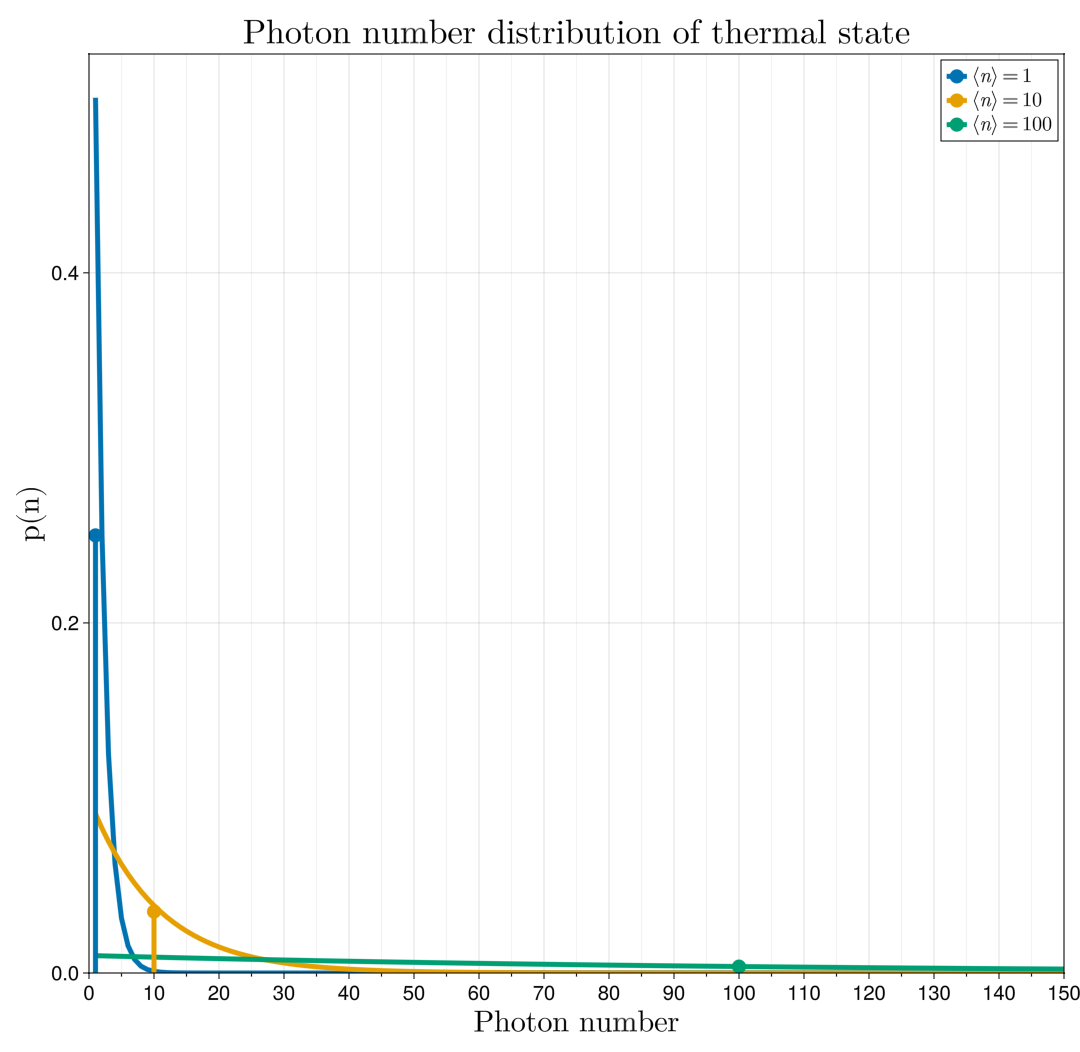
\includegraphics[width=0.8\textwidth]{imgs/fig_thermal.png}
    %\caption{Caption}
    %\label{fig:enter-label}
\end{figure}


\paragraph{About plotting the photon number distribution.}
Since the photon distributions of the coherent and Fock states can be described with well-known distributions and with useful properties where the relation between the expected value and the variance with the distribution is direct, there was no challenge into plotting the photon number distribution given the expected value.
However, for the coherent state, the expected value is bounded to the following physical parameters, $\omega$ and $T$.
Hence we need an expression for $\omega$ and $T$ given the expected value of the photon number.
From the previous result with $x=\hbar\omega/k_BT$,
\begin{align*}
    \expval{\hat{n}} &= \frac{e^{-x}}{1-e^{-x}} \\
    \frac{1-e^{-x}}{e^{-x}} &= \frac{1}{\expval{\hat{n}}} \\
    e^{x}\qty(1-e^{-x}) &= \frac{1}{\expval{\hat{n}}} \\
    e^{x}-1 &= \frac{1}{\expval{\hat{n}}} \\
    x &= \ln\qty[\frac{1}{\expval{\hat{n}}}+1] \\
    \frac{\omega}{T} &= \frac{k_B}{\hbar}\ln\qty[\frac{1}{\expval{\hat{n}}}+1].
\end{align*}
Now, with this expression, we can determine the ratio between the angular frequency and the temperature given the expected value of the photon number, hence, we can set the photon number distribution.



\section{Problem 2} Let the operators $\hata_i$ and $\hatad_i$, for $i=1,2$, form two sets of creation and annihilation operators that satisfy the commutation relations:
\begin{gather*}
   \commutator{\hata_i}{\hatad_j}=\delta_{ij},\qquad 
   \commutator{\hatad_i}{\hatad_j}=0,\qquad
   \commutator{\hata_i}{\hata_j}=0.
\end{gather*}
Let us define two new sets of creation and annihilation operators $\hat{b}^\dagger_i$ and $\hat{b}_i$, for $i=1,2$, which also follow the same commutation relations such that
\begin{gather*}
    \begin{pmatrix}
        \hata_1 \\ \hatad_2
    \end{pmatrix}
    =
    \begin{pmatrix}
        u & \upsilon \\ \upsilon & u
    \end{pmatrix}
    \begin{pmatrix}
        \hat{b}_1 \\ \hat{b}^\dagger_2
    \end{pmatrix}.
\end{gather*}
What relationship must the real numbers $u$ and $\upsilon$ satisfy?

Taking into account that the operators $\hat{b}_i, \hat{b}^\dagger_i$ have the same commutation relations of $\hata_i,\hatad_j$ we can start by expanding the matrix relation between them and use the commutation relationships to find the restrictions of the matrix elements.
Expanding the matrix relation we get the following system of equations,
\begin{align*}
    \hata_i &= u\hat{b}_i + \upsilon\hat{b}^\dagger_j \\
    \hatad_j &= \upsilon\hat{b}_i + u\hat{b}^\dagger_j .
\end{align*}

Now we can find a restriction by applying the commutator relationship between $\hatad_j$ and $\hata_i$,
\begin{align*}
    \commutator{\hata_1}{\hatad_2} &=  \qty[\qty(u\hat{b}_i + \upsilon\hat{b}^\dagger_j)\qty(\upsilon\hat{b}_i + u\hat{b}^\dagger_j)] - \qty[\qty(\upsilon\hat{b}_i + u\hat{b}^\dagger_j)\qty(u\hat{b}_i + \upsilon\hat{b}^\dagger_j)] \\
    &=  u\hat{b}_i\upsilon\hat{b}_i
        +u\hat{b}_iu\hat{b}^\dagger_j
        +\upsilon\hat{b}^\dagger_j\upsilon\hat{b}_i
        +\upsilon\hat{b}^\dagger_ju\hat{b}^\dagger_j
        -\upsilon\hat{b}_iu\hat{b}_i
        -\upsilon\hat{b}_i\upsilon\hat{b}^\dagger_j
        -u\hat{b}^\dagger_ju\hat{b}_i
        -u\hat{b}^\dagger_j\upsilon\hat{b}^\dagger_j \\
    &=  \qty(u\hat{b}_i\upsilon\hat{b}_i-\upsilon\hat{b}_iu\hat{b}_i)
        +\qty(u\hat{b}_iu\hat{b}^\dagger_j-u\hat{b}^\dagger_ju\hat{b}_i)
        +\qty(\upsilon\hat{b}^\dagger_j\upsilon\hat{b}_i-\upsilon\hat{b}_i\upsilon\hat{b}^\dagger_j)
       +\qty(\upsilon\hat{b}^\dagger_ju\hat{b}^\dagger_j -u\hat{b}^\dagger_j\upsilon\hat{b}^\dagger_j) \\
    &=  \cancelto{0}{u\upsilon\commutator{\hat{b}_i}{\hat{b}_i}}
        +u^2\commutator{\hat{b}_i}{\hat{b}^\dagger_j}
        +\upsilon^2\commutator{\hat{b}^\dagger_j}{\hat{b}_i}
        +\cancelto{0}{u\upsilon\commutator{\hat{b}^\dagger_j}{\hat{b}^\dagger_j}}
\end{align*}

Since $\commutator{\hata_i}{\hatad_j}=\delta_{ij}=\commutator{\hat{b}_i}{\hat{b}^\dagger_j}$, therefore $\commutator{\hat{b}_i}{\hat{b}^\dagger_j}=-\commutator{\hat{b}^\dagger_j}{\hat{b}_i}=-\delta_{ij}$, hence,
\begin{align*}
    \commutator{\hata_1}{\hatad_2} &= u^2\commutator{\hat{b}_i}{\hat{b}^\dagger_j} +\upsilon^2\commutator{\hat{b}^\dagger_j}{\hat{b}_i} \\
                       \delta_{ij} &= u^2\delta_{ij} - \upsilon^2\delta_{ij} \\
                       1 &= u^2 - \upsilon^2.
\end{align*}

This result tells us that the relation between the matrix elements needs to satisfy a hyperbola relation.

\section{Problem 3}

An electric field has an equal probability of $1/3$ to be found in each of the states $\ket{0},~\ket{2}$ and the superposition $4\ket{0}+3\ket{1}$ (before normalization).
Find the corresponding density matrix $\hat{\rho}$.

For this problem, we recall the definition of the density matrix with the projection operator
\begin{gather*}
    \hat{\rho} = \sum_n p_n\op{\psi_n}.
\end{gather*}
Taking into account the given states and probability we can expand the sum,
\begin{align*}
    \hat{\rho}  &= \frac{1}{3}\op{0} + \frac{1}{3}\op{2} + \frac{1}{3}\qty(\frac{4}{5}\ket{0}+\frac{3}{5}\ket{1})\qty(\frac{4}{5}\bra{0}+\frac{3}{5}\bra{1}) \\
        &= \frac{1}{3}\op{0} + \frac{1}{3}\op{2} 
            + \frac{1}{3}\left(
                \frac{16}{25}\op{0}{0}
                +\frac{12}{25}\op{0}{1}
                +\frac{12}{25}\op{1}{0}
                +\frac{9}{25}\op{1}{1}
                %\frac{4}{5}\bra{0}+\frac{3}{5}\bra{1}
                \right) \\
        &=\frac{41}{75}\op{0}+\frac{3}{25}\op{1}+\frac{1}{3}\op{2}+\frac{4}{25}\op{0}{1}+\frac{4}{25}\op{1}{0}.
\end{align*}

With this information, we can construct the density matrix,
\begin{gather*}
    \hat{\rho} =
        \begin{pmatrix}
            41/75 & 4/25 & 0 \\
            4/25 & 3/25 & 0 \\
            0 & 0 & 1/3
        \end{pmatrix}
        .
\end{gather*}

\section{Problem 4}

Do eigenstates of $\hatad$ exist?
If yes, so, what is their decomposition in the Fock state basis?

If we want to find the eigenstates of any operator, we establish the eigenvalue problem, \[\hatad\ket{\psi} = \lambda\ket{\psi}.\]
Rewriting the equation in a Fock state basis ($\ket{\psi}=\sum c_n\ket{n}$) and applying the previous result of $\hatad\ket{n}=\sqrt{n+1}\ket{n+1}$, we get
\begin{gather*}
    \hatad\ket{\psi} =\lambda\qty(\sum_{n=0}^\infty c_n\ket{n}) =\sum_{n=0}^\infty c_n\sqrt{n+1}\ket{n+1},
\end{gather*}
allowing us to establish the following restriction,
\begin{gather*}
    \lambda\qty(\sum_{n=0}^\infty c_n\ket{n}) - \sum_{n=0}^\infty c_n\sqrt{n+1}\ket{n+1} = 0.
\end{gather*}
Trying to solve for the coefficients $c_n$, we construct the following equation,
\begin{gather*}
    \lambda c_n\ket{n} - c_n\sqrt{n+1}\ket{n+1} = 0.
\end{gather*}
Since lambda cannot be a trivial solution, we need to apply the restriction to the coefficients $c_n$.
However, the only way the equation can be fulfilled will be if $c_n=0$, which tells us that there are no eigenstates of $\hatad$.
Also, if we start to analyze a recurrence relation between the coefficients, they cannot be normalized; therefore, we cannot use them.


%\section{Problem 5}

%A bright squeezed state result from the application of a squeezing operator to a coherent state.
%It is defined as: \[\ket{r,\alpha}=\hat{S}(r)\ket{\alpha},\] where the squeezing operator is defined as $\hat{S}(r)=\exp\qty[r/2\qty(\hata^{2}-\hatad^{2})].$
%Find the uncertainty of a bright squeezed state in position and momentum quadratures.
%Does it retain the average photon number associated with the coherent state?
%What would be different if we defined the bright squeezed state as a displaced squeezed vacuum state instead?




\end{document}
